\subsection*{Writing, Graphs}
Describe the figures~\ref{fig:ielts_writing_graph_households_cars},~\ref{fig:ielts_writing_graph_households_recycling},~\ref{fig:ielts_writing_graph_ballmer_peak}.

\begin{figure}[H]
  \centering
    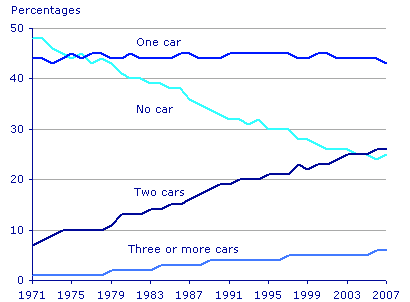
\includegraphics{ielts_writing_graph_households_cars}
  \caption{Households with regular use of a car, Great Britain}
  \label{fig:ielts_writing_graph_households_cars}
\end{figure}

\begin{answer}
The graph demonstrates the percentages of car ownership in households of Great Britain from 1971 to 2007. 
As we can see, the amount of households without a car decreased greatly, which correlates to the increased general welfare.

The percentage of households with two or more cars linearly increased through this period of time.

The percentage of households with one car generally remained the same over the years with a small fluctuations.
The dynamic of households with one car is negative while the number of households with two or more cars  increased, which means that more and more households are starting to buy a secondary cars.

The percentage of households without a car greatly decreased (from 48\% in 1971 to 25\% in 2007 reaching its bottom in 2006) but the dynamic seems to be changing to a positive value.
This dynamic is expected and tells us that there always will be some people that either don't want a car, or can't afford it yet.
\end{answer}

\begin{figure}[H]
  \centering
    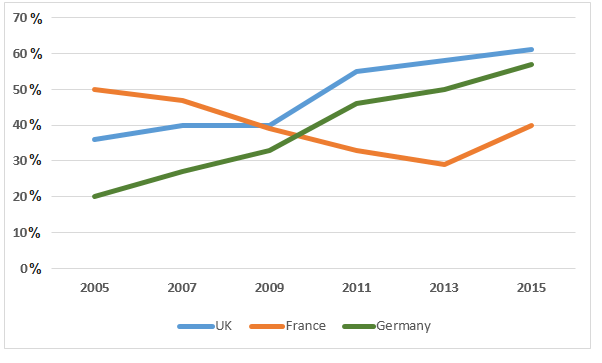
\includegraphics{ielts_writing_graph_households_recycling}
  \caption{Regional household recycling rates}
  \label{fig:ielts_writing_graph_households_recycling}
\end{figure}

\begin{answer}
The graph demonstrates changes of the recycling rates in households of United Kingdom, France and Germany from 2005 to 2015. 

Recycling rates of British and German households grew steadily though the whole period. 
The dynamics seem to be slowing, which means that rates will probably settle down somewhere around 70\%. 

In 2005 France had a major advantage in numbers with 50\% household wastes recycled comparing to UK's 37\% and Germany's 20\%. 
From 2005 and 2007 French rates decreased a bit and in 2007 began to fall rapidly reaching its bottom in 2013 with 29\%. 
After 2013 French rates began to rise regaining 11\% in 2 years.
The dynamic of French recycling rates is positive so the rates will catch up with British and German ones very soon.  
\end{answer}

\begin{figure}[H]
  \centering
    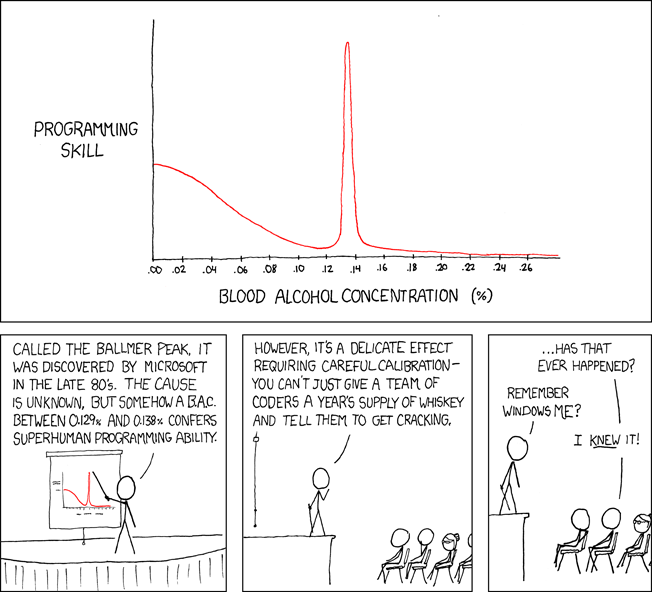
\includegraphics[width=\textwidth]{ielts_writing_graph_ballmer_peak}
  \caption{Ballmer peak, \texttt{https://xkcd.com/323/}}
  \label{fig:ielts_writing_graph_ballmer_peak}
\end{figure}

\begin{answer}
The graph looks similar to the Gaussian distribution with single high and dense peak at 0.139\% percents that more than doubles the normal programming ability.  

This peak is at very high blood alcohol concentration, which is strange, cause that much of alcohol causes far less muscle control than normal, slowed thinking and very little judgment/reasoning skills. 

The effects of the blood alcohol concentration probably result in a programmer who is not held back by his team's rules and can design an exceptional software architecture.
\end{answer}
